% ========================================
%	Header einbinden
% ========================================

\documentclass[bibtotoc,titlepage]{scrartcl}

% Deutsche Spracheinstellungen
\usepackage[ngerman,german]{babel, varioref}
\usepackage[T1]{fontenc}
\usepackage[utf8]{inputenc}

%\usepackage{marvosym}

\usepackage{amsfonts}
\usepackage{amssymb}
\usepackage{amsmath}
\usepackage{amscd}
\usepackage{amstext}

\usepackage{longtable}

%\usepackage{bibgerm}

\usepackage{footnpag}

\usepackage{ifthen}                 %%% package for conditionals in TeX
\usepackage[amssymb]{SIunits}
%Für textumflossene Bilder und Tablellen
%\usepackage{floatflt} - veraltet

%Für Testzwecke aktivieren, zeigt labels und refs im Text an.
%\usepackage{showkeys}

% Abstand zwischen zwei Absätzen nach DIN (1,5 Zeilen)
% \setlength{\parskip}{1.5ex plus0.5ex minus0.5ex}

% Einrückung am Anfang eines neuen Absatzes nach DIN (keine)
%\setlength{\parindent}{0pt}

% Ränder definieren
% \setlength{\oddsidemargin}{0.3cm}
% \setlength{\textwidth}{15.6cm}

% bessere Bildunterschriften
%\usepackage[center]{caption2}


% Problemlösungen beim Umgang mit Gleitumgebungen
\usepackage{float}

% Nummeriert bis zur Strukturstufe 3 (also <section>, <subsection> und <subsubsection>)
%\setcounter{secnumdepth}{3}

% Führt das Inhaltsverzeichnis bis zur Strukturstufe 3
%\setcounter{tocdepth}{3}
\usepackage[version=3]{mhchem}
	\mhchemoptions{minus-sidebearing-left=0.06em, minus-sidebearing-right=0.11em}
\usepackage{exscale}

\newenvironment{dsm} {\begin{displaymath}} {\end{displaymath}}
\newenvironment{vars} {\begin{center}\scriptsize} {\normalsize \end{center}}


\newcommand {\en} {\varepsilon_0}               % Epsilon-Null aus der Elektrodynamik
\newcommand {\lap} {\; \mathbf{\Delta}}         % Laplace-Operator
\newcommand {\R} { \mathbb{R} }                 % Menge der reellen Zahlen
\newcommand {\e} { \ \mathbf{e} }               % Eulersche Zahl
\renewcommand {\i} { \mathbf{i} }               % komplexe Zahl i
\newcommand {\N} { \mathbb{N} }                 % Menge der nat. Zahlen
\newcommand {\C} { \mathbb{C} }                 % Menge der kompl. Zahlen
\newcommand {\Z} { \mathbb{Z} }                 % Menge der kompl. Zahlen
\newcommand {\limi}[1]{\lim_{#1 \rightarrow \infty}} % Limes unendlich
\newcommand {\sumi}[1]{\sum_{#1=0}^\infty}
\newcommand {\rot} {\; \mathrm{rot} \,}         % Rotation
\newcommand {\grad} {\; \mathrm{grad} \,}       % Gradient
\newcommand {\dive} {\; \mathrm{div} \,}        % Divergenz
\newcommand {\dx} {\; \mathrm{d} }              % Differential d
\newcommand {\cotanh} {\; \mathrm{cotanh} \,}   %Cotangenshyperbolicus
\newcommand {\asinh} {\; \mathrm{areasinh} \,}  %Area-Sinus-Hyp.
\newcommand {\acosh} {\; \mathrm{areacosh} \,}  %Area-Cosinus-H.
\newcommand {\atanh} {\; \mathrm{areatanh} \,}  %Area Tangens-H.
\newcommand {\acoth} {\; \mathrm{areacoth} \,}  % Area-cotangens
\newcommand {\Sp} {\; \mathrm{Sp} \,}
\newcommand {\mbe} {\stackrel{\text{!}}{=}}     %Must Be Equal
\newcommand{\qed} { \hfill $\square$\\}
\renewcommand{\i} {\imath}
\def\captionsngerman{\def\figurename{\textbf{Abb.}}}

%%%%%%%%%%%%%%%%%%%%%%%%%%%%%%%%%%%%%%%%%%%%%%%%%%%%%%%%%%%%%%%%%%%%%%%%%%%%
% SWITCH FOR PDFLATEX or LATEX
%%%%%%%%%%%%%%%%%%%%%%%%%%%%%%%%%%%%%%%%%%%%%%%%%%%%%%%%%%%%%%%%%%%%%%%%%%%%
%%%
\ifx\pdfoutput\undefined %%%%%%%%%%%%%%%%%%%%%%%%%%%%%%%%%%%%%%%%% LATEX %%%
%%%
\usepackage[dvips]{graphicx}       %%% graphics for dvips
\DeclareGraphicsExtensions{.eps,.ps}   %%% standard extension for included graphics
\usepackage[ps2pdf]{thumbpdf}      %%% thumbnails for ps2pdf
\usepackage[ps2pdf,                %%% hyper-references for ps2pdf
bookmarks=true,%                   %%% generate bookmarks ...
bookmarksnumbered=true,%           %%% ... with numbers
hypertexnames=false,%              %%% needed for correct links to figures !!!
breaklinks=true,%                  %%% breaks lines, but links are very small
linkbordercolor={0 0 1},%          %%% blue frames around links
pdfborder={0 0 112.0}]{hyperref}%  %%% border-width of frames
%                                      will be multiplied with 0.009 by ps2pdf
%
\hypersetup{ pdfauthor   = {Hannes Franke; Julius Tilly},
pdftitle    = {V301 Innenwiderstand und Leistungsanpassung}, pdfsubject  = {Protokoll FP}, pdfkeywords = {V301, Innenwiderstand, Leistungsanpassung},
pdfcreator  = {LaTeX with hyperref package}, pdfproducer = {dvips
+ ps2pdf} }
%%%
\else %%%%%%%%%%%%%%%%%%%%%%%%%%%%%%%%%%%%%%%%%%%%%%%%%%%%%%%%%% PDFLATEX %%%
%%%
\usepackage[pdftex]{graphicx}      %%% graphics for pdfLaTeX
\DeclareGraphicsExtensions{.pdf}   %%% standard extension for included graphics
\usepackage[pdftex]{thumbpdf}      %%% thumbnails for pdflatex
\usepackage[pdftex,                %%% hyper-references for pdflatex
bookmarks=true,%                   %%% generate bookmarks ...
bookmarksnumbered=true,%           %%% ... with numbers
hypertexnames=false,%              %%% needed for correct links to figures !!!
breaklinks=true,%                  %%% break links if exceeding a single line
linkbordercolor={0 0 1},
linktocpage]{hyperref} %%% blue frames around links
%                                  %%% pdfborder={0 0 1} is the default
\hypersetup{
pdftitle    = {V301 Innenwiderstand und Leistungsanpassung}, 
pdfsubject  = {Protokoll AP}, 
pdfkeywords = {V301, Innenwiderstand, Leistungsanpassung},
pdfsubject  = {Protokoll AP},
pdfkeywords = {V301, Innenwiderstand, Leistungsanpassung}}
%                                  %%% pdfcreator, pdfproducer,
%                                      and CreationDate are automatically set
%                                      by pdflatex !!!
\pdfadjustspacing=1                %%% force LaTeX-like character spacing
\usepackage{epstopdf}
%
\fi %%%%%%%%%%%%%%%%%%%%%%%%%%%%%%%%%%%%%%%%%%%%%%%%%%% END OF CONDITION %%%
%%%%%%%%%%%%%%%%%%%%%%%%%%%%%%%%%%%%%%%%%%%%%%%%%%%%%%%%%%%%%%%%%%%%%%%%%%%%
% seitliche Tabellen und Abbildungen
%\usepackage{rotating}
\usepackage{ae}
\usepackage{
  array,
  booktabs,
  dcolumn
}
\makeatletter 
  \renewenvironment{figure}[1][] {% 
    \ifthenelse{\equal{#1}{}}{% 
      \@float{figure} 
    }{% 
      \@float{figure}[#1]% 
    }% 
    \centering 
  }{% 
    \end@float 
  } 
  \makeatother 


  \makeatletter 
  \renewenvironment{table}[1][] {% 
    \ifthenelse{\equal{#1}{}}{% 
      \@float{table} 
    }{% 
      \@float{table}[#1]% 
    }% 
    \centering 
  }{% 
    \end@float 
  } 
  \makeatother 
%\usepackage{listings}
%\lstloadlanguages{[Visual]Basic}
%\allowdisplaybreaks[1]
%\usepackage{hycap}
%\usepackage{fancyunits}


% ========================================
%	Angaben für das Titelblatt
% ========================================

\title{Versuch 500 - Der Photo-Effekt\\				% Titel des Versuchs 
\large TU Dortmund, Fakultät Physik\\ 
\normalsize Anfänger-Praktikum}

\author{Jan Adam\\			% Name Praktikumspartner A
{\small \href{jan.adam@tu-dortmund.de}{jan.adam@tu-dortmund.de}}	% Erzeugt interaktiven einen Link
\and						% um einen weiteren Author hinzuzfügen
Dimitrios Skodras\\					% Name Praktikumspartner B
{\small \href{dimitrios.skodras@tu-dortmund.de}{dimitrios.skodras@tu-dortmund.de}}		% Erzeugt interaktiven einen Link
}
\date{18. April 2013}				% Das Datum der Versuchsdurchführung

% ========================================
%	Das Dokument beginnt
% ========================================

\begin{document}

% ========================================
%	Titelblatt erzeugen
% ========================================

\maketitle					% Jetzt wird die Titelseite erzeugt
\thispagestyle{empty} 				% Weder Kopfzeile noch Fußzeile

% ========================================
%	Der Vorspann
% ========================================

%\newpage					% Wenn Verzeichnisse auf einer neuen Seite beginnen sollen
%\pagestyle{empty}				% Weder Kopf- noch Fußzeile für Verzeichnisse

\tableofcontents

%\newpage					% eine neue Seite
%\thispagestyle{empty}				% Weder Kopf- noch Fußzeile für Verzeichnisse
%\listoffigures					% Abbildungsverzeichnis

%\newpage					% eine neue Seite
%\thispagestyle{empty}				% Weder Kopf- noch Fußzeile für Verzeichnisse
%\listoftables					% Tabellenverzeichnis
\newpage					% eine neue Seite


% ========================================
%	Kapitel
% ========================================

\section{Theorie}
\setcounter{page}{1}
\subsection{Grundlagen zum Photoeffekt}
Der Photoeffekt, oder auch lichtelektrischer Effekt, ist ein Phänomen, bei welchem Photonen Elektronen aus Metalloberflächen herauslösen.
Das Wellenmodell hat lange Zeit das Wesen des Lichts gut beschreiben können, doch hieran scheitert es. Albert Einstein konnte 1905 die
Problematik durch die Zuweisung korpuskularer Eigenschaften an die Lichtquanten lösen. In Abbildung \ref{pic_photo} ist dies stilistisch gezeigt. Völlig korrekt wird sie durch Berechnungen aus
der Quantenelektrodynamik beschrieben, jedoch reicht die Betrachtung des Teilchenmodells für die Zwecke dieses Versuchs völlig aus.

\begin{figure}[H]
 
\begin{tikzpicture}[line cap=round,line join=round,>=triangle 45,x=0.7cm,y=0.7cm]
\clip(-2.96,-6.75) rectangle (15.68,6.42);
\draw [line width=1.2pt] (2,5)-- (9,5);
\draw [line width=1.2pt] (9,-1)-- (2,-1);
\draw [shift={(4,2)},line width=1.2pt]  plot[domain=2.16:4.12,variable=\t]({1*3.61*cos(\t r)+0*3.61*sin(\t r)},{0*3.61*cos(\t r)+1*3.61*sin(\t r)});
\draw [shift={(7,2)},line width=1.2pt]  plot[domain=-0.98:0.98,variable=\t]({1*3.61*cos(\t r)+0*3.61*sin(\t r)},{0*3.61*cos(\t r)+1*3.61*sin(\t r)});
\draw [line width=2.4pt] (2,4)-- (2,0);
\draw [line width=2.4pt] (9,4)-- (9,0);
\draw [line width=1.2pt] (2,2)-- (-2,2);
\draw [->,line width=1.2pt] (2,2) -- (8,1);
\draw [shift={(2.26,2.26)}] plot[domain=0.79:3.93,variable=\t]({1*0.37*cos(\t r)+0*0.37*sin(\t r)},{0*0.37*cos(\t r)+1*0.37*sin(\t r)});
\draw [shift={(2.76,2.76)}] plot[domain=-2.36:0.79,variable=\t]({1*0.34*cos(\t r)+0*0.34*sin(\t r)},{0*0.34*cos(\t r)+1*0.34*sin(\t r)});
\draw [shift={(3.26,3.26)}] plot[domain=0.79:3.93,variable=\t]({1*0.36*cos(\t r)+0*0.36*sin(\t r)},{0*0.36*cos(\t r)+1*0.36*sin(\t r)});
\draw [shift={(3.76,3.76)}] plot[domain=-2.36:0.79,variable=\t]({1*0.35*cos(\t r)+0*0.35*sin(\t r)},{0*0.35*cos(\t r)+1*0.35*sin(\t r)});
\draw [shift={(4.26,4.26)}] plot[domain=0.79:3.93,variable=\t]({1*0.36*cos(\t r)+0*0.36*sin(\t r)},{0*0.36*cos(\t r)+1*0.36*sin(\t r)});
\draw [shift={(4.76,4.76)}] plot[domain=-2.36:0.79,variable=\t]({1*0.35*cos(\t r)+0*0.35*sin(\t r)},{0*0.35*cos(\t r)+1*0.35*sin(\t r)});
\draw [shift={(5.24,5.24)}] plot[domain=0.79:3.93,variable=\t]({1*0.34*cos(\t r)+0*0.34*sin(\t r)},{0*0.34*cos(\t r)+1*0.34*sin(\t r)});
\draw [shift={(5.74,5.74)}] plot[domain=-2.36:0.79,variable=\t]({1*0.37*cos(\t r)+0*0.37*sin(\t r)},{0*0.37*cos(\t r)+1*0.37*sin(\t r)});
\draw [->,line width=1.2pt] (1.91,2.15) -- (2,2);
\draw [line width=1.2pt] (9,2)-- (13,2);
\draw [line width=1.2pt] (13,2)-- (13,-5);
\draw [line width=1.2pt] (-2,2)-- (-2,-5);
\draw [line width=1.2pt] (8,-5) circle (1cm);
\draw [line width=1.2pt] (3,-5) circle (1cm);
\draw [line width=1.2pt] (4.5,-5)-- (6.5,-5);
\draw [line width=1.2pt] (9.5,-5)-- (13,-5);
\draw [line width=1.2pt] (-2,-5)-- (1.5,-5);
\draw [->,line width=1.2pt] (6.5,-6.5) -- (9.5,-3.5);
\draw [->,line width=1.2pt] (6,-2) -- (13,-2);
\draw [->,line width=1.2pt] (4,-2) -- (-2,-2);
\draw [line width=1.2pt] (2.5,-4.66)-- (3.5,-4.66);
\draw [line width=1.2pt] (2.5,-5.33)-- (3.5,-5.33);
\draw (4.71,-1.63) node[anchor=north west] {$U$};
\draw (4.28,-5.74) node[anchor=north west] {$+$};
\draw (1.15,-5.74) node[anchor=north west] {$-$};
\draw (9.42,-5.64) node[anchor=north west] {$I$};
\draw (6.33,6.2) node[anchor=north west] {$\hbar\,\omega$};
\draw (-2.96,4.78) node[anchor=north west] {$Photokathode$};
\draw (10.21,4.7) node[anchor=north west] {$Auffangelektrode$};
\draw (7.44,1.99) node[anchor=north west] {$e^-$};
\end{tikzpicture}
 \caption{Anordnung zum Photoeffekt}
 \label{pic_photo}
\end{figure}

Hierbei trifft ein Photon der Energie $\hbar\omega$ auf das Metall und löst ein Elektron $e^-$ mit einer Bindungsenergie $A_k$ heraus
und überträgt den Überschuss in Form von kinetischer Energie

\begin{align}
 \hbar\omega = h\nu = E_{kin} + A_k.
 \label{eq_photo}
\end{align}

Aus den Experimenten zum Photoeffekt haben sich folgende Gesetzmäßigkeiten herauskristallisiert:

\begin{enumerate}
 \item Es existiert eine Minimalfrequenz $\nu_{min}$, ab der der Photoeffekt überhaupt auftritt.
 \item Die Energie der Photoelektronen ist proportional zur Frequenz der Photonen.
 \item Die Zahl der herausgelösten Elektronen ist proportional zur Lichtintensität.
\end{enumerate}

\subsection{Die Gegenfeldmethode}
Da das Picoamperemeter lediglich feststellen kann, ob ein Elektron eintrifft, aber nichts über die Energie aussagen kann, wird ein
Gegenfeld erzeugt, um eben diese zu ermitteln. Lediglich die Elektronen, die genug kinetische Energie inne haben, sind in der Lage
das Gegenfeld bei einer Grenzspannung $U_g$ zu durchlaufen und zur Anode zu gelangen. Mit Gleichung \eqref{eq_photoerweitert} lassen sich grundsätzlich $A_k$ und 
$h/e_0$ errechnen.

\begin{align}
 h\nu = e_0 U_g + A_k
 \label{eq_photoerweitert}
\end{align}

Jedoch ist die Energie der Elektronen im Metal nicht einheitlich sondern unterliegt der Fermi-Dirac-Verteilung. Sie führt auf, dass
Elektronen eine Energie im Bereich von 0 und der Fermie-Energie $\zeta$ und bei endlicher Temperatur gar darüber haben. Das führt dazu,
dass Elektronen auch mehr Energie haben, als die Differenz von Photonenenergie und Austrittsarbeit zulässt. Unter bestimmten 
Voraussetzungen kann man annehmen, dass der Photostrom $I_{Ph}$ parabolisch mit der Bremsspannung $U$ zusammenhängt. 

\begin{align}
 I_{Ph} \propto U^2
 \label{eq_stromspannung}
\end{align}

\section{Durchführung}
\begin{figure}[H]
 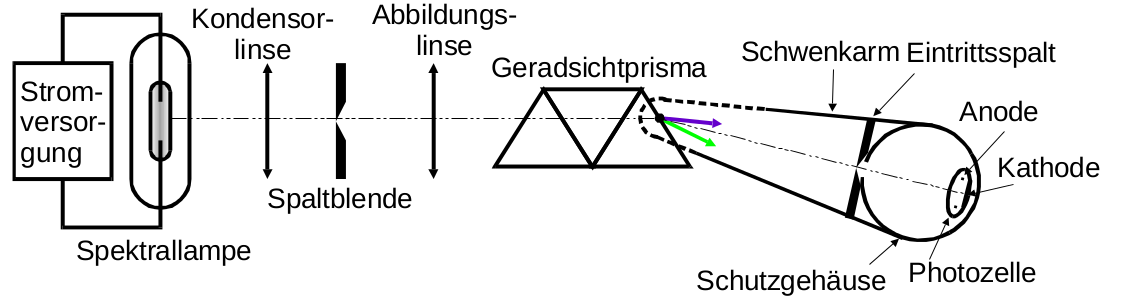
\includegraphics[width=\textwidth]{pics/Aufbau.png}
 \caption{Schematischer Aufbau der benutzten Apparatur}
 \label{pic_aufbau}
\end{figure}

In Abbildung \ref{pic_aufbau} ist der Versuchsaufbau dargestellt. Das Licht der Quecksilberlampe wird durch eine Kondensorlinse gebündelt,
trifft auf eine Spaltblende und wird von der Abbildungslinse auf das Geradsichtprisma fokussiert. Das Prisma sorgt für eine räumliche
Aufteilung der einzelnen Spektrallinien, welche eine Photokathode bestrahlen, die auf einem schwenkbaren Arm befestigt ist. Somit wird
Die Photokathode immer mit monochromatischem Licht beleuchtet. 

Für vier Spektrallinien wird der Photostrom in Abhängigkeit der Bremsspannung gemessen, welche in einem Bereich von -2V $\leq \,U \, \leq 2$V
liegt. Für die Wellenlänge $\lambda$ = 438,8 nm wird zusätzlich der Bereich von -20V $\leq \,U \, \leq$ 20V gegen den Photostrom gemessen.


\section{Auswertung}



Um die $I_{pk} \propto U^2$
Gesetzmäßigkeit nachzuweisen, wird die Wurzel des Stroms gegen die Spannung aufgetragen.

\begin{figure}[H]
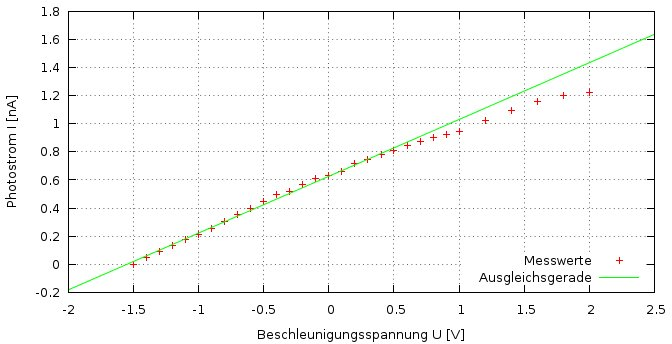
\includegraphics[width=0.8\textwidth]{pics/wurzel404.jpg}
\caption{Photostrom gegen die Spannung aufgetragen - 404,7nm}
\end{figure}

\begin{figure}[H]
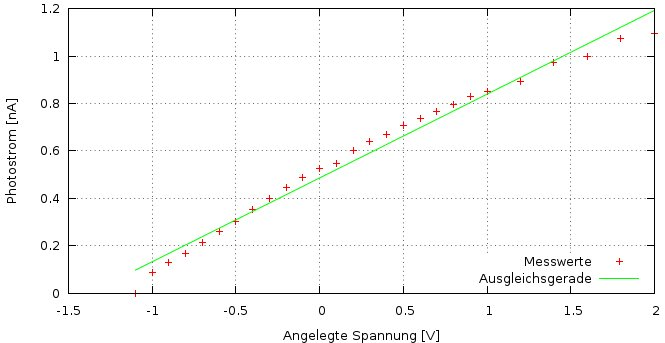
\includegraphics[width=0.8\textwidth]{pics/wurzel407.jpg}
\caption{Photostrom gegen die Spannung aufgetragen - 407,8nm}
\end{figure}
\newpage
Verwendet wurden dabei folgende Messwerte:
\renewcommand{\arraystretch}{.95}
\begin{table}[H]
\begin{tabular}{|c|c!{\vrule width 1.5pt} c|c!{\vrule width 1.5pt} c|c!{\vrule width 1.5pt} c|c|}
\hline
435.8nm &  & 404.7nm &  & 407.8nm & & 546.1nm & \\ \hline
V	&		A&		V&		A&	V&A			&V	&A \\ \hline
-1.0 & 0 	& -1.5 & 0 		& -1.1 & 0 		& -0.6&0 \\ \hline
-0.9 & 0.01 & -1.4 & 0.002 	& -1.0 & 0.008 	& -0.5&0 \\ \hline
-0.8 & 0.0025 & -1.3 & 0.008 & -0.9 & 0.017 & -0.4&0.003 \\ \hline
-0.7 & 0.007 & -1.2 & 0.018 & -0.8 & 0.028 & -0.3&0.014 \\ \hline
-0.6 & 0.0094 & -1.1 & 0.03 & -0.7 & 0.046 & -0.2&0.052 \\ \hline
-0.5 & 0.0198 & -1.0 & 0.046 & -0.6 & 0.068 & -0.1&0.12 \\ \hline
-0.4 & 0.022 & -0.9 & 0.066 & -0.5 & 0.091 & 0.0&0.17 \\ \hline
-0.3 & 0.028 & -0.8 & 0.094 & -0.4 & 0.125 & 0.1&0.26 \\ \hline
-0.2 & 0.036 & -0.7 & 0.125 & -0.3 & 0.16 & 0.2&0.34 \\ \hline
-0.1 & 0.045 & -0.6 & 0.16 & -0.2 & 0.2 & 0.3&0.42 \\ \hline
0.0 & 0.056 & -0.5 & 0.2 & -0.1 & 0.24 & 0.4&0.49 \\ \hline
0.1 & 0.065 & -0.4 & 0.0245 & 0.0 & 0.275 & 0.5&0.56 \\ \hline
0.2 & 0.076 & -0.3 & 0.265 & 0.1 & 0.3 & 0.6&0.62 \\ \hline
0.3 & 0.085 & -0.2 & 0.32 & 0.2 & 0.36 & 0.7&0.66 \\ \hline
0.4 & 0.09 & -0.1 & 0.37 & 0.3 & 0.41 & 0.8&0.7 \\ \hline
0.5 & 0.11 & 0.0 & 0.4 & 0.4 & 0.45 & 0.9&0.74 \\ \hline
0.6 & 0.125 & 0.1 & 0.44 & 0.5 & 0.5 & 1.0&0.78 \\ \hline
0.7 & 0.135 & 0.2 & 0.52 & 0.6 & 0.54 & 1.2&0.87 \\ \hline
0.8 & 0.145 & 0.3 & 0.56 & 0.7 & 0.59 & 1.4&0.93 \\ \hline
0.9 & 0.155 & 0.4 & 0.61 & 0.8 & 0.63 & 1.6&1.08 \\ \hline
1.0 & 0.17 & 0.5 & 0.66 & 0.9 & 0.69 & 1.8&1.15 \\ \hline
1.1 & 0.175 & 0.6 & 0.72 & 1.0 & 0.72 & 2.0&1.2 \\ \hline
1.2 & 0.18 & 0.7 & 0.77 & 1.2 & 0.8 &&  \\ \hline
1.3 & 0.185 & 0.8 & 0.81 & 1.4 & 0.95 &&  \\ \hline
1.4 & 0.205 & 0.9 & 0.86 & 1.6 & 1 &  &\\ \hline
1.5 & 0.215 & 1.0 & 0.89 & 1.8 & 1.15 &&  \\ \hline
2.0 & 0.26 & 1.2 & 1.05 & 2.0 & 1.2 && \\ \hline
3.0 & 0.37 & 1.4 & 1.2 &  & && \\ \hline
4.0 & 0.44 & 1.6 & 1.35 &  && & \\ \hline
5.0 & 0.54 & 1.8 & 1.45 &  && & \\ \hline
6.0 & 0.6 & 2.0 & 1.5 &  && & \\ \hline
7.0 & 0.64 & & & & && \\ \hline
8.0 & 0.66 & & & & && \\ \hline
9.0 & 0.74 & & & & && \\ \hline
10.0 & 0.78 & & & & & &\\ \hline
12.0 & 0.82 &  & & & &&\\ \hline
14.0 & 0.89 & & & & & &\\ \hline
16.0 & 0.94 & & & & & &\\ \hline
18.0 & 1 & 	& & & & &\\ \hline
\end{tabular}
\renewcommand{\arraystretch}{1}
\caption{Messwerte}
\end{table}

\begin{figure}[H]
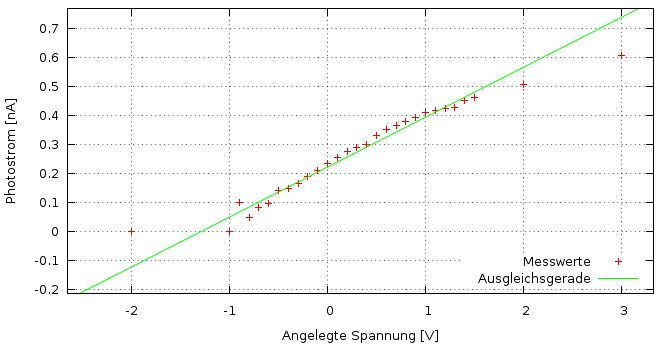
\includegraphics[width=0.8\textwidth]{pics/wurzel4358.jpg}
\caption{Photostrom gegen die Spannung aufgetragen - 435,8nm}
\end{figure}

\begin{figure}[H]
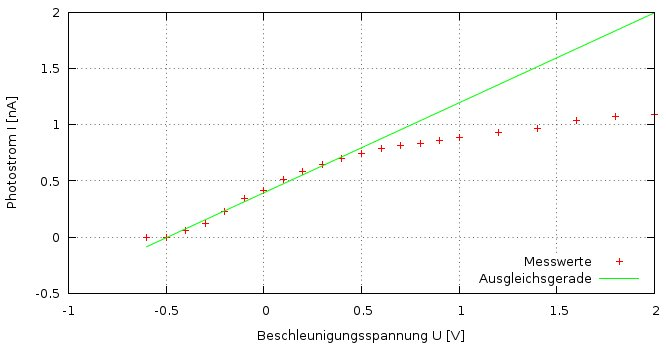
\includegraphics[width=0.8\textwidth]{pics/wurzel546.jpg}
\caption{Photostrom gegen die Spannung aufgetragen - 546,1nm}
\end{figure}

Als Y-Achsenabschnitt liest sich dann die Spannung ab, ab der ein Photostrom gemessen werden kann:

\begin{align*}
0.600\text{V}	=	404.7\text{nm}\\
0.486\text{V}	=	407.8\text{nm}\\
0.222\text{V}	=	435.8\text{nm}\\
0.386\text{V}	=	546.1\text{nm}\\
\end{align*}

Für Licht der Wellenlänge 435,8nm wurde der Photostrom über einen weiteren Spannungsbereich aufgenommen. Der Plot ergab folgendes Diagram:

\begin{figure}[H]
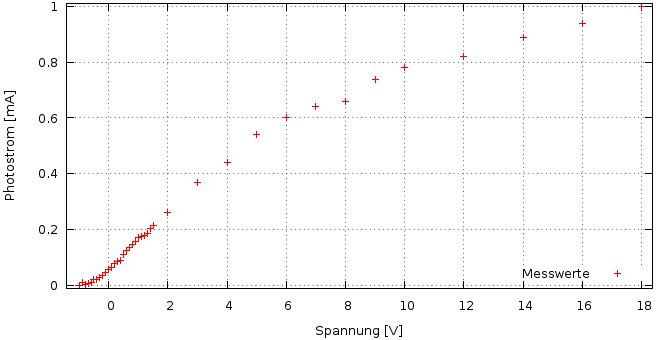
\includegraphics[width=0.6\textwidth]{pics/gesamt.jpg}
\caption{Photostrom und Spannung für 435,8nm}
\end{figure}

Zunächst lässt sich festhalten, dass selbst bei negativen Beschleunigungsspannung bereits ein schwacher Phtotostrom messbar ist. Die liegt daran, dass die Elektronen im Metal, eine der Dirac-Verteilung entsprechende Energieverteilung haben und die Energie für einige der Elektronen ausreicht, um das Metal spontan zu verlassen und gegen das Gegenfeld anzulaufen. Der Kurvenverlauf in diesem Bereich stimmt auch sehr gut mit der Dirac-Kurve überein.\
Sobald die Spannung größer wird, beginnt die Kurve zu steigen. Die liegt daran, dass zunehmend mehr Elektronen vom elektrischen Feld eingefangen und zur Anode transportiert werden. Die Steigung der Kurve ist hier nahezu linear.\\
Bei höheren Spannung stellt sich schließlich eine Sättigung des Stromes ein. Dies kennzeichnet den Bereich, ab dem quasi alle Elektronen, die das Metal verlassen auch durch das elektrische Feld zur Anode gelangen. Bei noch größeren Spannungen kann ihre Anzahl nicht weiter steigen.

Die vier Werte, die sich aus der Gegenspannung und der Frequenz zusammensetzen, ergeben leider keine schöne Gerade. Möglicherweise hat sich aus den vorherigen Rechnungen ein Folgefehler eingeschlichen, so dass diese Auswertung kein brauchbares Ergebnis liefert. (Ich werde das nochmal am Wochenende nachprüfen.)

\begin{figure}[H]
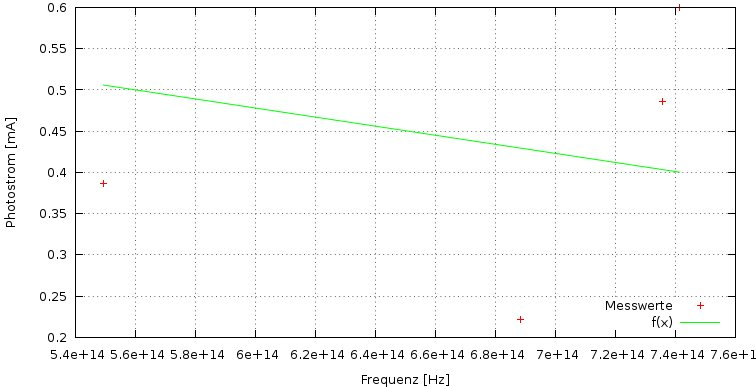
\includegraphics[width=0.6\textwidth]{pics/4werte.jpg}
\caption{Gegenspannung gegen Frequenz}
\end{figure} 
%\section{Diskussion}

% ========================================
%	Literaturverzeichnis
% ========================================

%\bibliographystyle{plainnat}			% Bibliographie-Style auswählen
%\bibliography{BIBDATEI}			% Literaturverzeichnis

% ========================================
%	Das Dokument endent
% ========================================

\end{document}
